\chapter{Example of initialisation sequence for grid-nesting run}\label{a:sequence}
\begin{itemize}
\item The following initialisation and gridnesting sequence is shown here for
 three models, model~2 included in model~1, and model~3 included in model~2
(figure (\ref{seq1})):
\begin{enumerate}
\item
{\bf PREP\_PGD}: this program is run as many time as the number of models:
\begin{itemize}
\item one physiographic data file for the model~1 (definition of projection, resolution, domain)
\item one physiographic data file for the model~2 (same projection, definition of resolution, domain)
\item one physiographic data file for the model~3 (same projection, definition of resolution, domain)
\end{itemize}
\item
{\bf PREP\_NEST\_PGD}: this program checks all the three PGD files at the same
 time, and imposes the conformity between them.
\item
{\bf extractecmwf} or {\bf extractarpege}: it extracts the surface
and altitude fields for one date, for model~1.
The extraction must be done separately for each date and time (for
the initial file and each of the coupling file of model~1).
\item 
{\bf PREP\_REAL\_CASE}: this program is running several times, for the initial
file and the coupling files of model~1.
\item 
{\bf MESONH}: this step is {\bf optional}. If you do not wish to start 
all the models at the same time, you can decide to run the model~1 before
the model~2 starts.
\item
{\bf ZOOM\_PGD}: this step is {\bf optional}. If you want to start the model~2 
on a smaller domain than the one of the PGD file defined at
steps 1 and 2 for the model~2, you must use this program.
\item
{\bf SPAWNING}: when you want to start the model~2, you must use this
program to compute the horizontal interpolations from the model~1 to 
the model~2. It is used only once for the initialisation of model~2.
\item 
{\bf PREP\_REAL\_CASE}: It is used only once, to compute the
initial file for the model~2. {\bf Do not change the vertical grid}.
\item 
{\bf MESONH}: again, this step is {\bf optional}. If you do not wish to start 
model~3 at the same time as model~2, you can decide to run
the models 1 and 2 alone before.
\item
{\bf ZOOM\_PGD}: again, this step is {\bf optional}. If you want to start the
 model~3 on a smaller domain than the one of the PGD file defined at
steps 1 and 2 for the model~3, you must use this program.
\item
{\bf SPAWNING}: when you want to start the model 3, you must use this
program to compute the horizontal interpolations from the model~2 to the 
model~3. It is used only once for the initialisation of model~3.
\item 
{\bf PREP\_REAL\_CASE}: It is used only once, to compute the initial
file for the model~3. {\bf Do not change the vertical grid}.
\item 
{\bf MESONH}: here is now your complete nested run.
\end{enumerate} 
\begin{figure}[htb]
\vspace*{1.cm}
%\hspace*{-1.2cm}
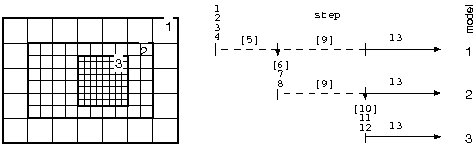
\includegraphics[width=15.cm]{annexes/seq1}
%\vspace*{-0.4cm}
\caption{Exemple of a grid-nesting simulation with 3 nested models
\label{seq1}}
\end{figure}
\newpage
\item The following initialisation and gridnesting sequence is shown here for
 three models, model~2 included in model~1, and model~3 included in model~1.
Model~3 has the same resolution as model~2 and is started after model~2
 to follow atmospheric system
(figure (\ref{seq2})):
\begin{enumerate}
\item
{\bf PREP\_PGD}: 
\begin{itemize}
\item one physiographic data file for the model 1 (definition of projection, resolution, domain)
\item one physiographic data file for the models 2 and 3 (same projection,
definition of resolution, domain)
\end{itemize} 
\item
{\bf PREP\_NEST\_PGD}: this program checks all the two PGD files at the same 
time, and imposes the conformity between them.
\item
{\bf extractecmwf} or {\bf extractarpege}: it extracts the surface
and altitude fields for one date, for model 1.
The extraction must be done separately for each date and time (for
the initial file and each of the coupling file of model~1).
\item 
{\bf PREP\_REAL\_CASE}: this program is run several times, for the initial
file and the coupling files of model~1.
\item 
{\bf MESONH}: this step is {\bf optional}. If you do not wish to start 
all the models at the same time, you can decide to run the model~1 before
the model~2 starts.
\item
{\bf ZOOM\_PGD}: Since the second PGD file was done for models
2 and 3, you have to zoom it on the domain of model~2 with this program.
\item
{\bf SPAWNING}: when you want to start the model~2, you must use this
program to compute the horizontal interpolations from the model 1 to the model
2. It is used only once for the initialisation of model~2.
\item 
{\bf PREP\_REAL\_CASE}: It is used only once, to compute the
initial file for the model~2. {\bf Do not change the vertical grid}.
\item 
{\bf MESONH}: here is your complete nested run with model~1 and model~2.
\item
{\bf ZOOM\_PGD}: Since the second PGD file was done for the models
2 and 3, you have to zoom it on the domain of model~3 with this program.
The domain of model~3 has a common zone with the one of model~2.
\item
{\bf SPAWNING}: when you want to start the model 3, you must use this
program to compute the horizontal interpolations from the model 1 and to 
use the fields of model 2 in the common domain.
It is used only once for the initialisation of model~3.
\item 
{\bf PREP\_REAL\_CASE}: It is used only once, to compute the
initial file for the model~3. {\bf Do not change the vertical grid}.
\item 
{\bf MESONH}: here is the nested run with model~1 and model~3.

\end{enumerate} 

\begin{figure}[htb]
\vspace*{1.cm}
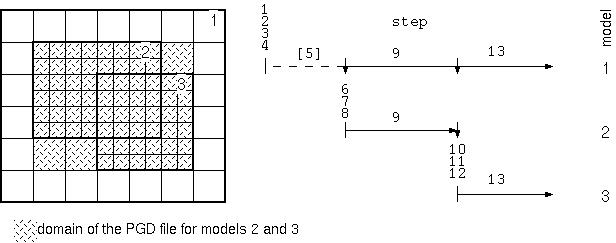
\includegraphics[width=15.cm]{annexes/seq2}
\caption{Exemple of a grid-nesting simulation with 3 nested models (the domain
of the 2 finest models has the same resolution and a common zone to follow
atmospheric system).
\label{seq2}}
\end{figure}
\end{itemize} 
